% Generated by tools/render_numerical_results.py; values come from audit JSON.
\subsection{Independent numerical verification and discontinuities}
\label{sec:numerical_revision}

The revised code was checked against independently assembled stationary
face balances, a continuum transport solution and adaptive backward
differentiation formula (BDF) integration of the coupled semi-discrete
transport--sorption equations. These checks address equation solving and
discretisation separately from a mass ledger. The complete integrated test
suite is reported separately; the focused checks below address independent
oracles, source discontinuities and exact reuse of equivalent tile states.

For a short nonlinear test, the reference column was set to eight cells and
capacity $10^{-5}$~kg/kg, so that breakthrough occurs within fourteen days.
This is an accelerated verification problem, not a revised material
calibration. Concentration and sorbed-profile errors were normalised by
$10^{-3}$~kg/m$^3$ and capacity, respectively, and compared at daily marks.
The reference uses SciPy~1.18.1's variable-order BDF integration with relative
tolerance $2\times10^{-9}$ and absolute tolerance $10^{-14}$.\citep{scipy_solve_ivp}
Table~\ref{tab:independent-temporal} reports the maximum normalised
profile error, not a fitted coefficient or an assumed precision.


\begin{table}[htbp]\centering\small
\caption{Convergence of the nonlinear column to independent adaptive BDF integration in the accelerated verification problem.}\label{tab:independent-temporal}
\begin{tabular}{rr}\toprule
Step (h) & Maximum normalised profile error \\\midrule
6 & 0.0947294 \\
3 & 0.0534873 \\
1.5 & 0.03128 \\
\bottomrule\end{tabular}\end{table}


\begin{table}[htbp]\centering\small
\caption{Spatial refinement of the non-sorbing reference column against its continuum solution. The approximately halving error is consistent with first-order upwind transport.}\label{tab:independent-spatial}
\begin{tabular}{rr}\toprule
Layer cells & Relative stationary flux error (\%) \\\midrule
20 & 1.12686 \\
40 & 0.564771 \\
80 & 0.2825 \\
160 & 0.141248 \\
\bottomrule\end{tabular}\end{table}


The largest per-step mass residual in this nonlinear verification was $1.60308\times10^{-20}$~kg/m$^2$, with zero recorded clipping. The finite temporal errors in Table~\ref{tab:independent-temporal} show why conservation cannot establish accuracy. The runtime now refuses unconverged sorption branch masks with an instruction to reduce the step or increase the iteration limit.


Within-call reuse of exactly equivalent vertical tile states was also checked against independent per-tile advancement. Fourteen additional regression cases preserve complete step results, identities and independent arrays. A 30-day full-history comparison was bitwise identical across all result fields. One exploratory timing gave 2.14-fold speedup; the recorded repeat under concurrent workload gave 1.17-fold (6.62 versus 7.75~s). Runtime depends on workload; nine equivalent solver calls being reduced to one does not imply ninefold end-to-end acceleration. The benchmark artifact and reproduction script accompany the repository.


The exact discrete barrier also removes a mismatch in the former diagnostic:
the old continuum approximation double-counted a top half-cell resistance and
approximated advective bottom resistance. At the default clean state, the
corrected barrier flux is 2.1346\% higher for Pb and Hg and 2.7534\% higher for
Cu than that old comparison. This changes the interpretation of the plotted
barrier; it does not alter the transport trajectory or calibrate the material.

Two remaining types of abrupt behaviour have explicit causes. First, a step
in the prescribed source changes the denominator of
$1-J_{\mathrm{out}}/J_{\mathrm{bare}}$ immediately, whereas porewater storage
is continuous. A tenfold source decrease produces a tenfold instantaneous
increase in that residual ratio, followed by washout
(Figure~\ref{fig:reactive-numerical-audit}D). Such a ratio dip is compatible
with a conserving solver. Second, the capacity-lock law itself is
discontinuous: an exactly full cell is held, but a cell just below capacity
can desorb. In a six-hour, one-cell clean-water flush, an exactly full state
gives zero outgoing flux; starting at $q/Q=1-10^{-10}$ gives
$9.8426\times10^{-12}$~kg/m$^2$/s. This is an unvalidated constitutive
assumption retained explicitly, not evidence that real keratin exhibits that
switch. No plotted trajectory was smoothed to conceal these effects.


\begin{figure}[htbp]\centering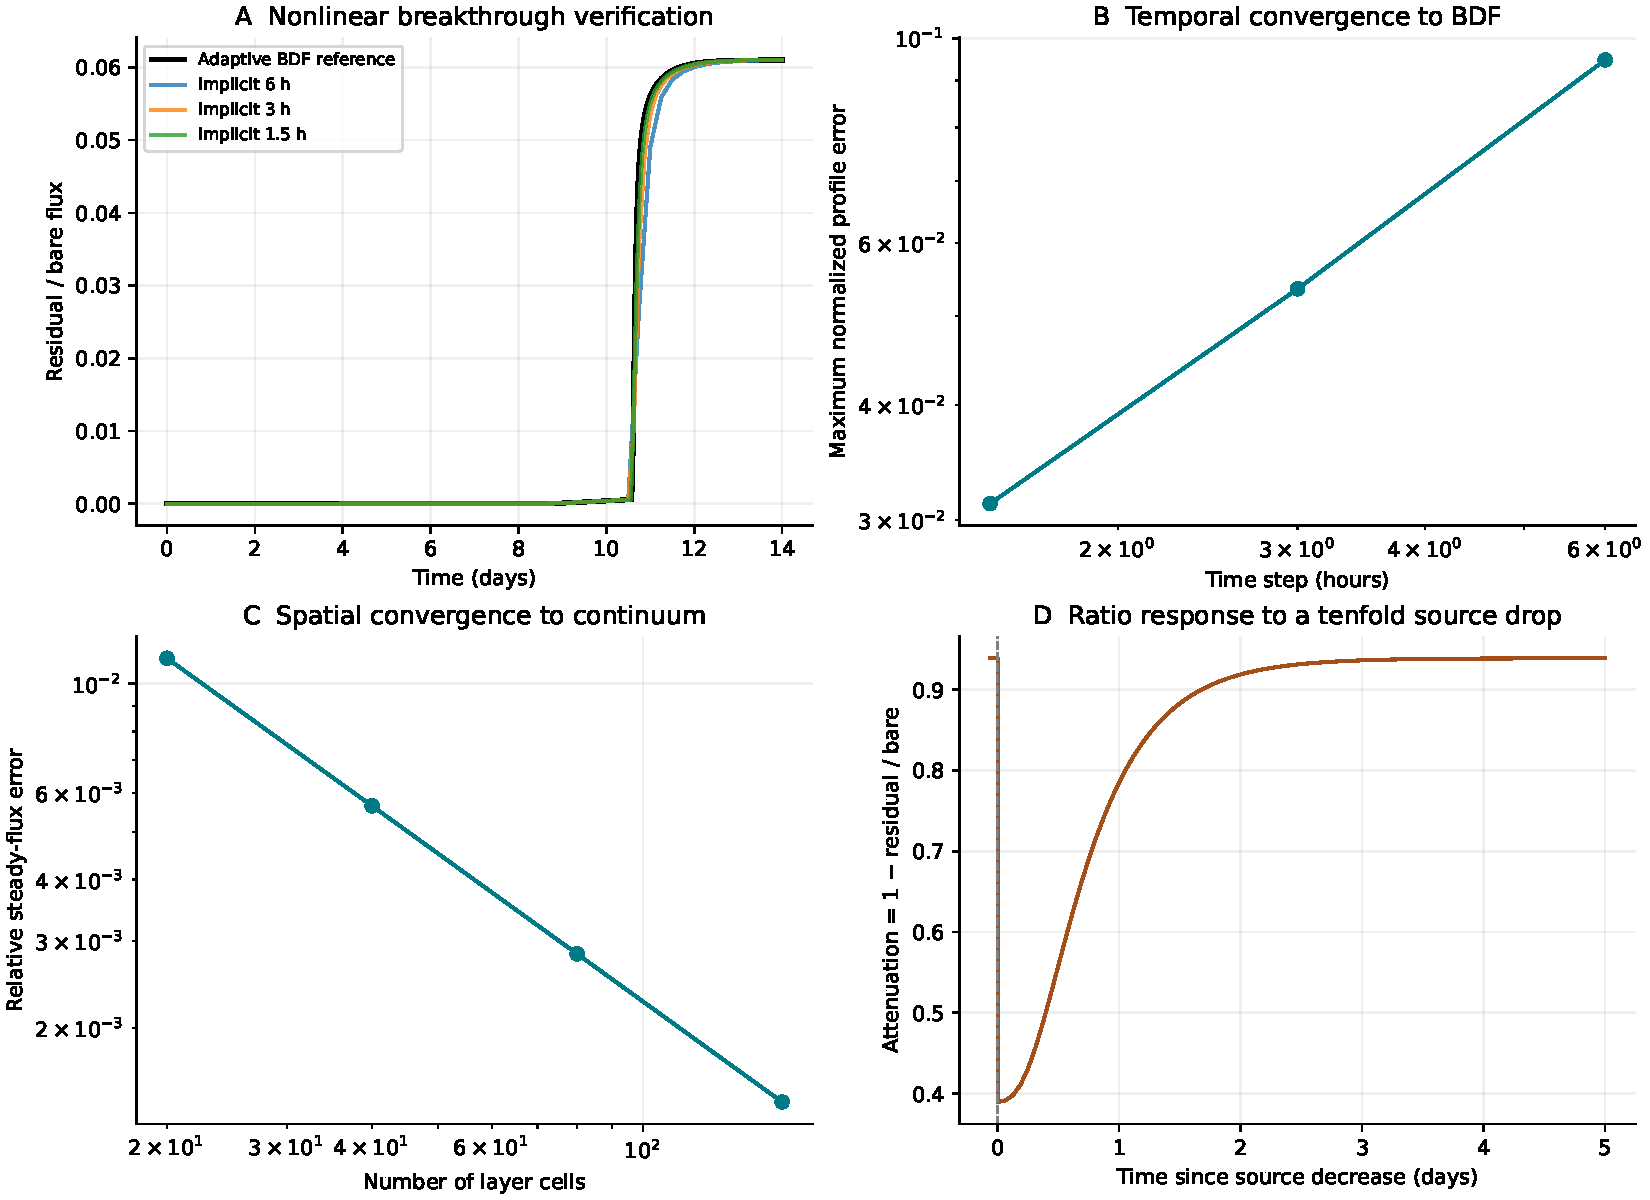
\includegraphics[width=\linewidth]{figures/reactive_numerical_audit.pdf}
\caption{Independent column verification and a forcing-induced ratio dip. A: nonlinear breakthrough against adaptive BDF; B: the maximum normalised profile error under time refinement; C: stationary flux error under spatial refinement; D: instantaneous ratio change and subsequent washout after a tenfold source decrease. The low-capacity test in A--B accelerates verification and is not a scenario material adjustment.}\label{fig:reactive-numerical-audit}\end{figure}


\subsection{Regenerated time-step, horizon and decision studies}
\label{sec:timescale_revision}

The following values were regenerated after the scientific corrections.
Attenuation refers to the whole-hotspot, area-mixed source, including bypass,
and each age is an actually simulated endpoint. The source hash, scenario
identifier and full-precision arrays accompany the manuscript in
\path{data/timescale_audit.json}; the executable study is
\path{tools/timescale_check.py} in the repository.


\begin{table}[htbp]\centering\small
\caption{Regenerated two-year temporal refinement. Source attenuation and the whole-hotspot water input have a different control volume from active column inventory.}\label{tab:revised-refinement}
\resizebox{\linewidth}{!}{\begin{tabular}{rrrrrr}\toprule
Step (h) & Pb attenuation & Pb occupancy & Active Pb (kg) & Pb into water (kg) & Relative imbalance \\\midrule
24 & 0.82725239 & 0.580811 & 8.94603 & 20.884 & $6.64\times10^{-14}$ \\
12 & 0.82723547 & 0.580935 & 8.94794 & 20.8902 & $7.95\times10^{-14}$ \\
6 & 0.8272271 & 0.580997 & 8.9489 & 20.8932 & $2.01\times10^{-14}$ \\
3 & 0.82722292 & 0.581028 & 8.94938 & 20.8948 & $1.95\times10^{-13}$ \\
1 & 0.82722013 & 0.581048 & 8.94969 & 20.8958 & $1.25\times10^{-13}$ \\
\bottomrule\end{tabular}}\end{table}


The terminal attenuation spread is $3.226\times10^{-5}$, and the default six-hour result differs from the finest tested step by $6.976\times10^{-6}$. These are measured sensitivities of these endpoint quantities, not error bounds for every transient feature or for the coastal field.


\begin{table}[htbp]\centering\small
\caption{Exact-age samples from one continuous trajectory through the longest horizon. Barrier attenuation uses the same instantaneous geometry, fouling and bypass as the transient source.}\label{tab:revised-horizon}
\resizebox{\linewidth}{!}{\begin{tabular}{rrrrrrrr}\toprule
Age (yr) & Pb attenuation & Hg attenuation & Cu attenuation & Pb barrier & Hg barrier & Cu barrier & Services \\\midrule
1 & 0.899333 & 0.919219 & 0.871295 & 0.871545 & 0.871545 & 0.871257 & 0 \\
2 & 0.827227 & 0.846831 & 0.819577 & 0.819748 & 0.819748 & 0.819536 & 0 \\
4 & 0.717464 & 0.724005 & 0.715906 & 0.715946 & 0.715946 & 0.715858 & 0 \\
8 & 0.594422 & 0.595379 & 0.594313 & 0.594324 & 0.594324 & 0.594313 & 0 \\
16 & 0.594324 & 0.594327 & 0.594313 & 0.594324 & 0.594324 & 0.594313 & 0 \\
\bottomrule\end{tabular}}\end{table}


Horizon dependence describes evolving storage and condition. The difference
between transient and stationary-barrier attenuation includes history and
dissolved storage; it is not a separately validated sorbent efficiency or a
service-life measurement.


\begin{table}[htbp]\centering\small
\caption{Coastal duration and tidal-phase sensitivity. Every run starts from clean water with the same exact one-year mat state; the source is fixed during the window. Integer-cycle endpoints provide an additional comparison at matching phases.}\label{tab:revised-window}
\resizebox{\linewidth}{!}{\begin{tabular}{rrrrrr}\toprule
Window (h) & Tidal cycles & Pb peak: mat (ng/L) & Pb peak: bare (ng/L) & Peak ratio & Source ratio \\\midrule
3 & 0.2415 & 17.6971 & 175.798 & 0.1006671 & 0.1006671 \\
6 & 0.4831 & 3.78804 & 37.6294 & 0.1006671 & 0.1006671 \\
12 & 0.9662 & 5.74824 & 57.1015 & 0.1006671 & 0.1006671 \\
24 & 1.932 & 6.03871 & 59.9869 & 0.1006671 & 0.1006671 \\
24.84 & 2 & 5.82456 & 57.8597 & 0.1006671 & 0.1006671 \\
37.26 & 3 & 5.84223 & 58.0352 & 0.1006671 & 0.1006671 \\
48 & 3.865 & 10.2414 & 101.735 & 0.1006671 & 0.1006671 \\
49.68 & 4 & 5.8281 & 57.8948 & 0.1006671 & 0.1006671 \\
\bottomrule\end{tabular}}\end{table}


The with-mat terminal Pb maximum spans 3.78804--17.6971~ng/L, while the with/bare peak ratio spans 0.10066706--0.10066706. A nearly invariant ratio can coexist with tide-dependent absolute peaks when a linear transport model is driven by proportional source fields.


These endpoint observations are not a monotonic steady-state convergence
sequence. Duration changes both spin-up and tidal phase, whereas matching
integer-cycle endpoints test approach to a periodic response. This finite set
does not prove that a periodic state has settled. A tide-dependent peak is not
by itself a solver defect; the separate discretisation study below measures
time-step and grid sensitivity under a fixed physical window and phase.


\begin{table}[htbp]\centering\small
\caption{Four-year decision-cadence comparison with a global observation calendar. Recommendations count individual returned recommendations, not necessarily distinct campaign dates.}\label{tab:revised-cadence}
\resizebox{\linewidth}{!}{\begin{tabular}{rrrrrr}\toprule
Review period (d) & Recommendations & Services & Observations & Pb attenuation & Assumed cost (EUR) \\\midrule
15 & 97 & 0 & 19593 & 0.717464 & 0 \\
30 & 48 & 0 & 19593 & 0.717464 & 0 \\
90 & 16 & 0 & 19593 & 0.717464 & 0 \\
180 & 8 & 0 & 19593 & 0.717464 & 0 \\
365 & 4 & 0 & 19593 & 0.717464 & 0 \\
\bottomrule\end{tabular}}\end{table}


The station/time/parameter/method calendar hashes are identical across these cadence runs. This check compares observation calendars, not noisy measured values or the subset available at any particular decision. Cadence determines when existing evidence is reviewed; it must not generate additional samples.


\begin{figure}[htbp]\centering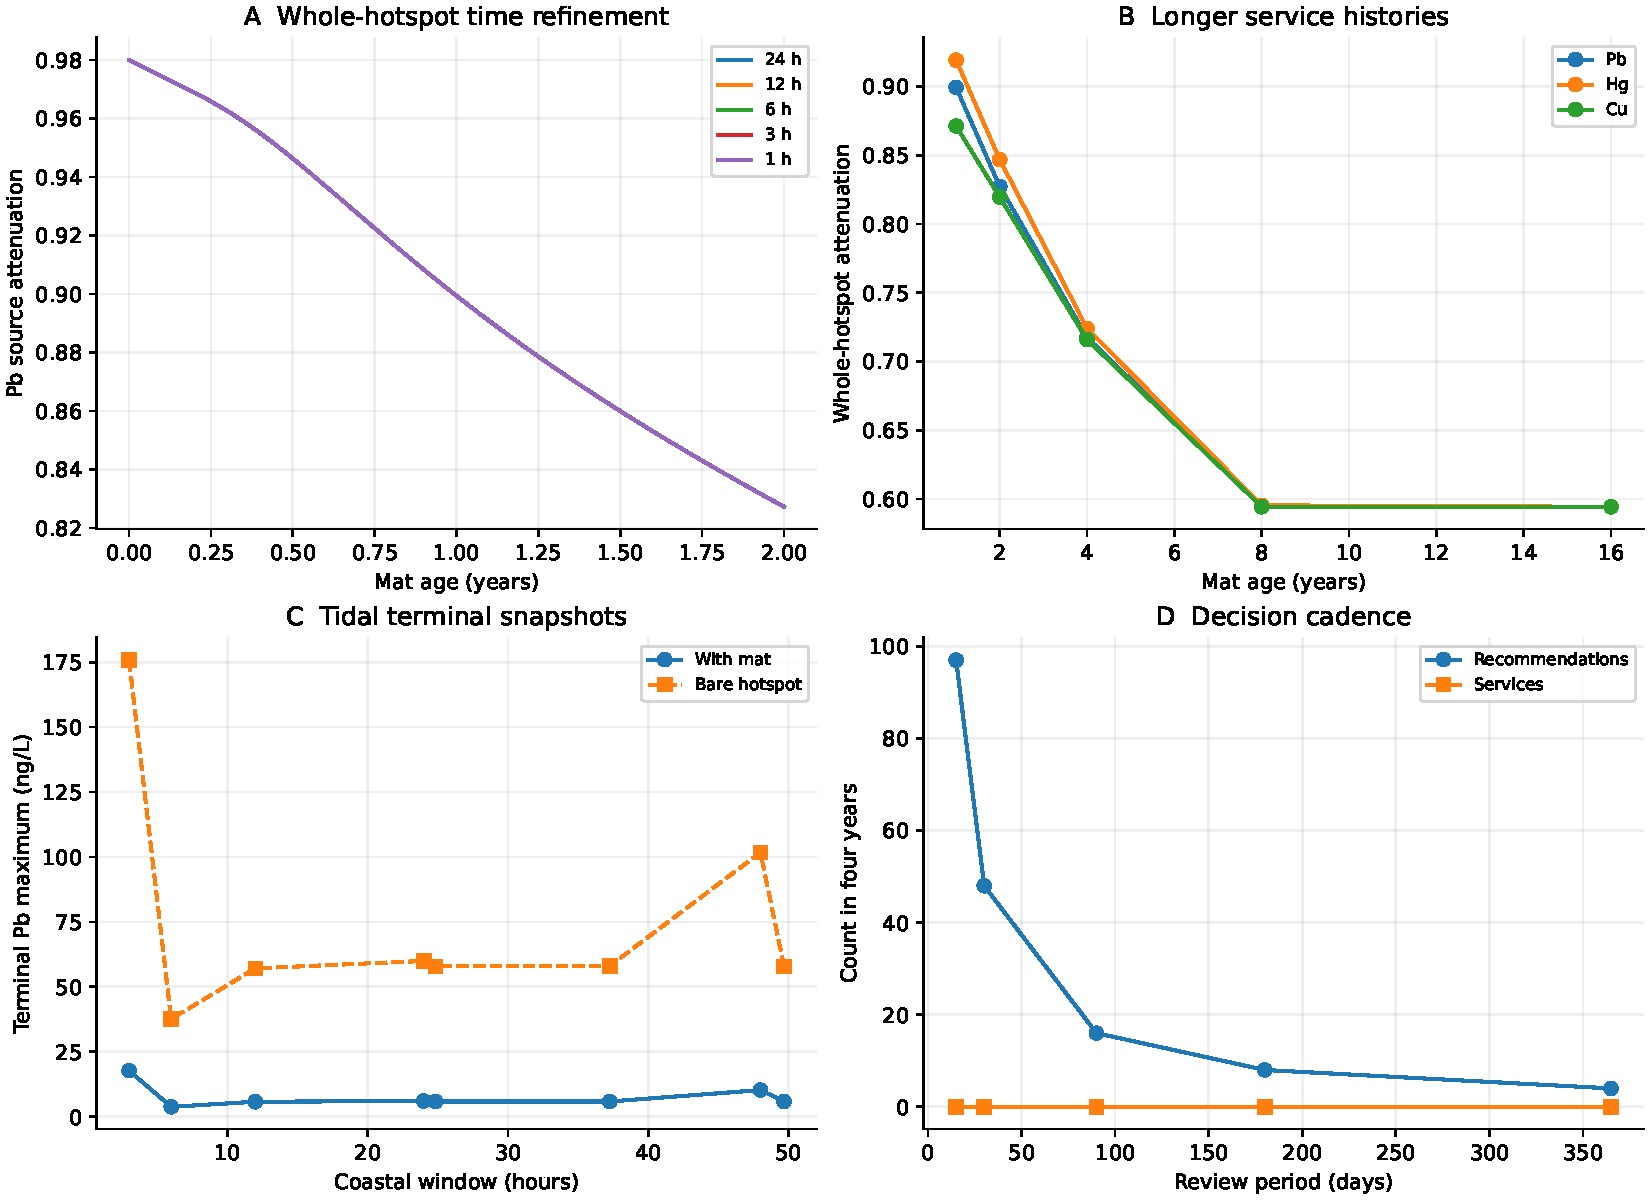
\includegraphics[width=\linewidth]{figures/timescale_audit.pdf}
\caption{Regenerated scenario studies: A, two-year whole-hotspot attenuation under time refinement; B, longer exact-age histories; C, terminal coastal maxima at different window lengths and tidal phases; D, recommendations and accepted services at different review cadences. Lines join computed samples without smoothing; the coarse horizon samples are not continuous observations.}\label{fig:timescale-audit}\end{figure}


\subsection{Coastal discretisation sensitivity}
\label{sec:coastal_refinement}

The coastal audit holds the $600\times400$~m physical domain, one-year mat
state, initial concentration, forcing phase, fixed source and 24-hour window
constant. Time steps of 600, 300 and 150~s use a 10-m grid; grids of 20, 10
and 5~m use a 150-s step. The hotspot and straight land edges align with all
three grids, avoiding a change in prescribed footprint area. The same FiPy
transport implementation is used.\citep{fipy2009}


\begin{table}[htbp]\centering\small
\caption{Fixed-window coastal time-step and grid refinement. These are numerical sensitivities rather than uncertainty intervals from material variability.}\label{tab:coastal-discretisation}
\resizebox{\linewidth}{!}{\begin{tabular}{rrrrrr}\toprule
Grid (m) & Step (s) & Pb peak: mat (ng/L) & Pb peak: bare (ng/L) & Peak ratio & Pb in water (kg) \\\midrule
10 & 600 & 6.03871 & 59.9869 & 0.1006671 & 0.000972618 \\
10 & 300 & 5.90376 & 58.6464 & 0.1006671 & 0.000868248 \\
10 & 150 & 5.86022 & 58.2138 & 0.1006671 & 0.00082418 \\
20 & 150 & 5.75969 & 57.2152 & 0.1006671 & 0.000845344 \\
5 & 150 & 5.88378 & 58.4479 & 0.1006671 & 0.000818459 \\
\bottomrule\end{tabular}}\end{table}


The 600-s versus 150-s terminal with-mat Pb peak difference at 10~m is 3.046\%; the 10-m versus 5-m difference at 150~s is -0.400\%. Each signed difference is expressed relative to the finer result. Coexisting temporal and spatial errors prevent these differences from being interpreted as bounds relative to an exact PDE solution. A stable source ratio or closed water ledger does not eliminate peak-concentration discretisation error.


For the remaining Pb inventory in the water, the corresponding differences are 18.010\% under time refinement and 0.699\% under grid refinement. The larger temporal sensitivity of this integrated field quantity further limits claims of coastal numerical accuracy based on a terminal peak alone.


\begin{figure}[htbp]\centering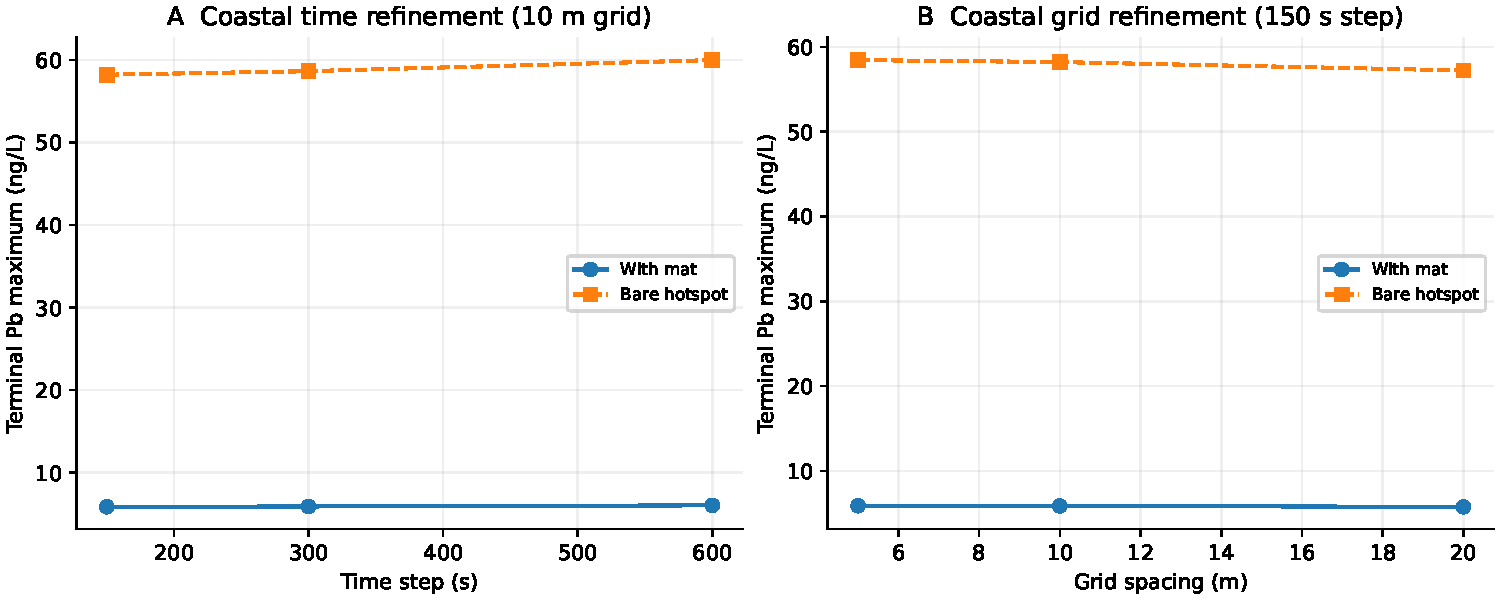
\includegraphics[width=\linewidth]{figures/coastal_discretisation_audit.pdf}
\caption{Coastal numerical sensitivity at a fixed one-year mat state and fixed 24-hour tidal window. Left: time-step refinement on the 10-m grid; right: grid refinement at 150 s. The relative with/bare source response may be more stable than either absolute terminal maximum.}\label{fig:coastal-discretisation-audit}\end{figure}
